\documentclass{beamer}

\usepackage{graphicx,hyperref,udesc,url}
\usepackage[utf8]{inputenc}
\usepackage[T1]{fontenc}
\usepackage{booktabs}
\usepackage[portuges]{babel}


\title[Project Euler]{Aventuras no Project Euler:}
\subtitle{Ou como eu ganhei uma tatuagem de graça}

\author[Renan S. Silva]{{\small \url{uber.renan@gmail.com}}}

\institute[UDESC]{Departamento de Ci\^encia da Computa\c{c}\~ao \\
    Centro de Ci\^encias e Tecnol\'ogias\\
Universidade do Estado de Santa Catarina}

\begin{document}

\begin{frame}
    \titlepage

\end{frame}

\section{Introdução}
\begin{frame}
    \frametitle{Quem Sou}

    \begin{itemize}
        \item Cursando o 7º semestre(4-8 Fase) do BCC
        \item Speedcuber
        \item Origamista
        \item IC na área de Otimização Combinatorial
    \end{itemize}
\end{frame}

\begin{frame}
    \frametitle{Project Euler}
    O que é?

    \begin{itemize}
        \item Começou com Colin Hughes (a.k.a euler) no \url{http://mathschallenge.net/} (RIP)
        \item Tornou-se um projeto própio em 2006.
        \item É uma série de problemas envolvendo matemática e computação.
        \item Todos os problemas podem ser resolvidos em menos de 1 minuto.
        \item 1 problema novo toda semana.
    \end{itemize}
\end{frame}

\begin{frame}
    \frametitle{Project Euler}

    \begin{center}
        \textit{
            "Project Euler exists to encourage, challenge, and develop the skills and enjoyment of anyone with an interest in the fascinating world of mathematics."
        }
    \end{center}
\end{frame}

\begin{frame}
    \frametitle{Números}

    \begin{itemize}
        \item 600000 membros inscritos
        \item 7950000 Problemas resolvidos
        \item Média de 13.3 por membro
        \item 82000 membros resolveram pelo menos 25 problemas (13.7\%)
        \item 60 membros resolveram 500 problemas ou mais (561 problemas ao todo)
    \end{itemize}

    Linguagens mais usadas: Python, C/C++, Java, C\#, Haskell
\end{frame}

\begin{frame}
    \frametitle{Mais números}

    \begin{figure}[htpb]
        \centering
        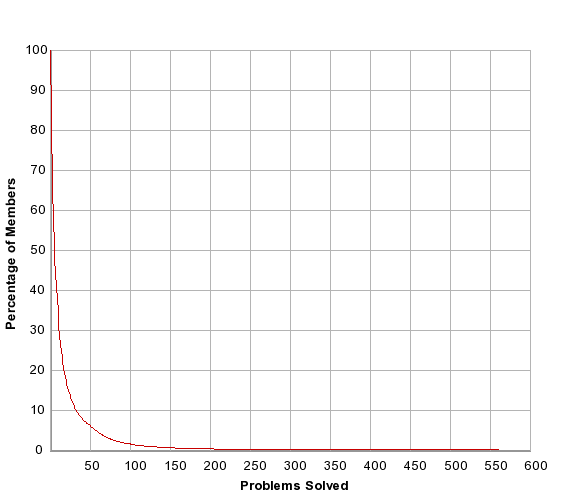
\includegraphics[width=0.8\linewidth]{images/graph1.png}
        \caption{images/Graph1}
        \label{fig:images/graph1}
    \end{figure}
\end{frame}

\begin{frame}
    \frametitle{Mais números}

    \begin{figure}[htpb]
        \centering
        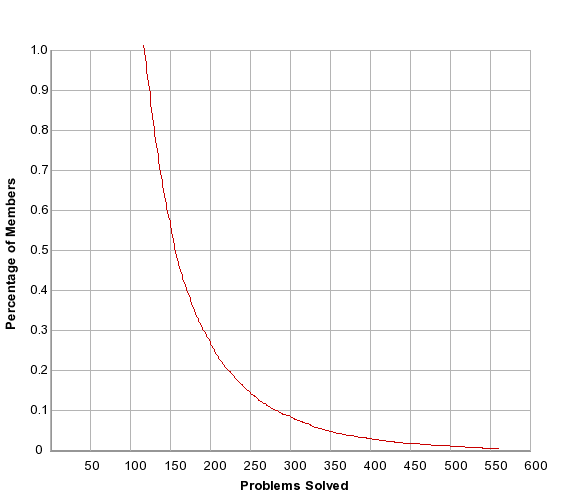
\includegraphics[width=0.8\linewidth]{images/graph2.png}
        \caption{images/Graph2}
        \label{fig:images/graph2}
    \end{figure}
\end{frame}

\begin{frame}
    \frametitle{Top 100}

    Top 100 de alguns países:

    \begin{table}[htpb]
        \centering
        \begin{tabular}{c c c}
            País             & Mínimo para o top 100 & Membros ativos \\ \hline \hline
            USA              & 256                   & 37527 \\
            Holanda          & 106                   & 3508 \\
            França           & 148                   & 4419 \\
            Russia           & 119                   & 4419 \\
            Brazil           & 35                    & 3110 \\
            República Tcheca & 37                    & 1087 \\
        \end{tabular}
    \end{table}
\end{frame}

\begin{frame}
    \frametitle{Ranking Brasileiro}
\begin{figure}[htpb]
    \centering
    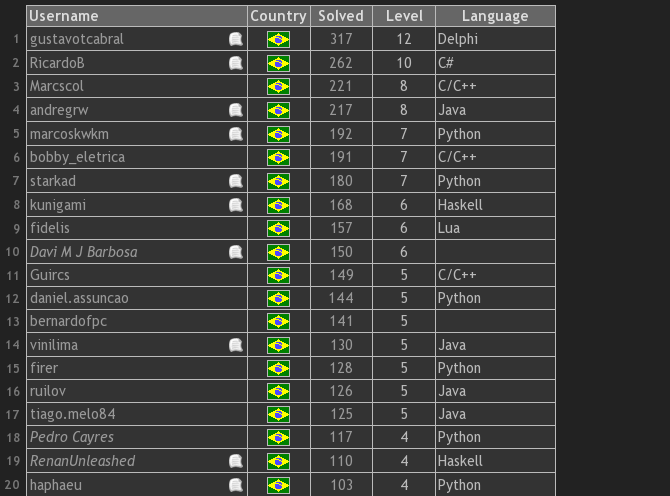
\includegraphics[width=0.8\linewidth]{images/top20_br.png}
\end{figure}
\end{frame}

\section{Problemas}

\begin{frame}
    \frametitle{Problema 1}
    \begin{center}
        \textit{
            If we list all the natural numbers below 10 that are multiples of 3 or 5, we get 3, 5, 6 and 9. The sum of these multiples is 23.
            Find the sum of all the multiples of 3 or 5 below 1000.
        }
    \end{center}

    Soluçao:
    \begin{center}
        \texttt{sum [ x|x<-[2..999], x `mod` 3 == 0 || x `mod`5 == 0 ]}
    \end{center}

\end{frame}

\begin{frame}
    \frametitle{Problema 5}

    \begin{center}
        \textit{
            2520 is the smallest number that can be divided by each of the numbers from 1 to 10 without any remainder.
            What is the smallest positive number that is evenly divisible by all of the numbers from 1 to 20?
        }
    \end{center}

    Soluçao:
    \begin{equation}
        \prod_{i=1}^{20} i
    \end{equation}
\end{frame}

\begin{frame}
    \frametitle{Problema 5}

    \begin{figure}[htpb]
        \centering
        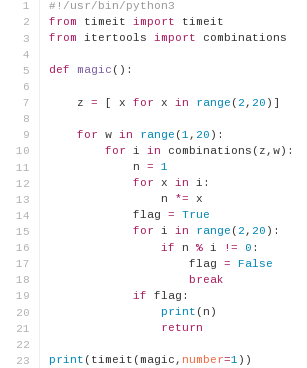
\includegraphics[width=0.4\linewidth]{images/prob5.png}
        \caption{Solução vergonhosa}
    \end{figure}

\end{frame}

\begin{frame}
    \frametitle{Problema 5}

    Solução de gente:

    \begin{center}
        $2^4 * 3^2 * 5 * 7 * 11 * 13 * 17 * 19$
    \end{center}

\end{frame}

\begin{frame}
    \frametitle{Problema 18}

    \begin{center}
        \textit{
            By starting at the top of the triangle below and moving to adjacent numbers on the row below, the maximum total from top to bottom is 23.
        }
        \begin{figure}[htpb]
            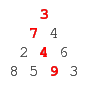
\includegraphics[width=0.2\linewidth]{images/p18_1.png}
        \end{figure}
        \textit{
            That is, 3 + 7 + 4 + 9 = 23.
            Find the maximum total from top to bottom of the triangle below:
            \footnotesize NOTE: As there are only 16384 routes, it is possible to solve this problem by trying every route. However, Problem 67, is the same challenge with a triangle containing one-hundred rows; it cannot be solved by brute force, and requires a clever method! ;o)
        }
    \end{center}

\end{frame}

\begin{frame}
    \frametitle{Problema 18}
    \begin{figure}[htpb]
        \centering
        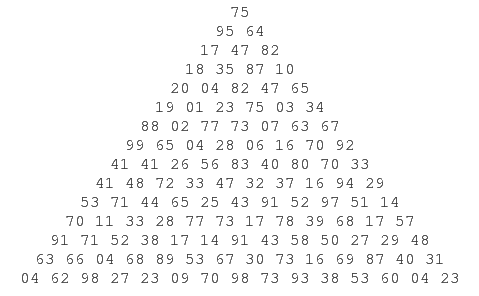
\includegraphics[width=0.8\linewidth]{images/p18_2.png}
    \end{figure}
\end{frame}

\begin{frame}
    \frametitle{Problema 18}
    \begin{figure}[htpb]
        \centering
        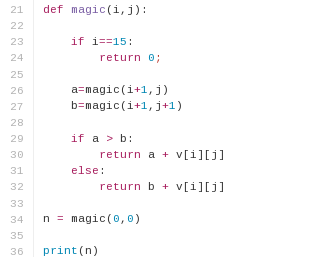
\includegraphics[width=0.5\linewidth]{images/prob18.png}
        \caption{Solução de força bruta}
    \end{figure}
\end{frame}

\begin{frame}
    \frametitle{Problema 67}

    \begin{center}
        \textit{
            By starting at the top of the triangle below and moving to adjacent numbers on the row below, the maximum total from top to bottom is 23.
        }
        \begin{figure}[htpb]
            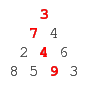
\includegraphics[width=0.2\linewidth]{images/p18_1.png}
        \end{figure}
        \textit{
            That is, 3 + 7 + 4 + 9 = 23.
            Find the maximum total from top to bottom in triangle.txt (right click and 'Save Link/Target As...'), a 15K text file containing a triangle with one-hundred rows.\\
        }
        \textit{
            \footnotesize NOTE: This is a much more difficult version of Problem 18. It is not possible to try every route to solve this problem, as there are 299 altogether! If you could check one trillion (1012) routes every second it would take over twenty billion years to check them all. There is an efficient algorithm to solve it. ;o)
        }
    \end{center}

\end{frame}

\begin{frame}
    \frametitle{Problema 67}

    \begin{figure}[htpb]
        \centering
        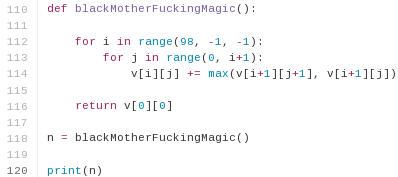
\includegraphics[width=0.8\linewidth]{images/prob67.png}
        \caption{Solução Uliziando PD}
    \end{figure}

\end{frame}

\begin{frame}
    \frametitle{Problema 75}

    \begin{center}
        \textit{
            \small It turns out that 12 cm is the smallest length of wire that can be bent to form an integer sided right angle triangle in exactly one way, but there are many more examples.\\
        }
        \begin{table}[htpb]
            \centering
            \begin{tabular}{c c c}
                12 cm: (3,4,5)   & 24 cm: (6,8,10)  & 30 cm: (5,12,13)\\
                36 cm: (9,12,15) & 40 cm: (8,15,17) & 48 cm: (12,16,20)\\
            \end{tabular}
        \end{table}
        \textit{
            \small In contrast, some lengths of wire, like 20 cm, cannot be bent to form an integer sided right angle triangle, and other lengths allow more than one solution to be found; for example, using 120 cm it is possible to form exactly three different integer sided right angle triangles.\\
        }
        \textit{
            120 cm: (30,40,50), (20,48,52), (24,45,51)\\
        }
        \textit{
            \small Given that L is the length of the wire, for how many values of L $\leq$ 1,500,000 can exactly one integer sided right angle triangle be formed?\\
        }
    \end{center}
\end{frame}

\begin{frame}
    \frametitle{Problema 75}

    Solução: Formula de Euclides (Elementos)

    \begin{align}
        a & = m^2 - n^2 \\
        b & = 2*m*n     \\
        c & = m^2 + n^2
    \end{align}

    onde $m$ e $n$ são coprimos, $m+n$ é ímpar e $n < m$. \\
    Para cara $(m, n)$ obtem-se uma tripla pitagorica.
\end{frame}

\begin{frame}
    \frametitle{Problema 75}

    \begin{figure}[htpb]
        \centering
        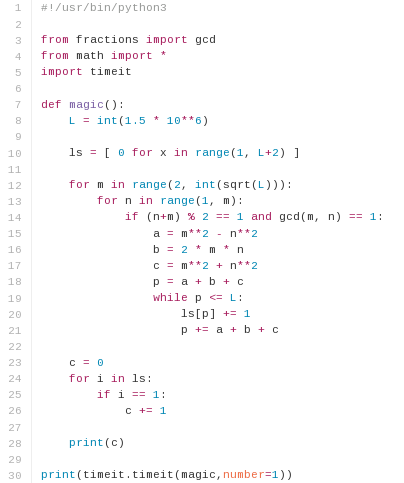
\includegraphics[height=0.75\textheight]{images/prob75.png}
        \caption{Solução do problema 75}
    \end{figure}
\end{frame}

\begin{frame}
    \frametitle{Problema 108}

    \begin{center}
        \textit{
            In the following equation x, y, and n are positive integers.
        }
    \end{center}

    \begin{equation}
        \frac{1}{x} + \frac{1}{y} = \frac{1}{n}
    \end{equation}

    \begin{center}
        \textit{
            For n = 4 there are exactly three distinct solutions:
        }
    \end{center}

    \begin{align}
        \frac{1}{5} + \frac{1}{20} & = \frac{1}{4} \\
        \frac{1}{6} + \frac{1}{12} & = \frac{1}{4} \\
        \frac{1}{8} + \frac{1}{8}  & = \frac{1}{4}
    \end{align}

    \begin{center}
        \textit{
            What is the least value of n for which the number of distinct solutions exceeds one-thousand?
        }
    \end{center}
\end{frame}

\begin{frame}
    \frametitle{Problema 108}

    Soluçao:
    \begin{equation}
        \frac{1}{x} + \frac{1}{y} = \frac{1}{n}
    \end{equation}
    seja $x=n+a$ e $y=n+b$
    \begin{align}
        \frac{1}{(n+a)} + \frac{1}{(n+b)} & = \frac{1}{n}        \\
        \frac{n+a + n+b}{(n+a)(n+b)}      & = \frac{1}{n}        \\
        n*(n+a+n+b)                       & = (n+a)(n+b)         \\
        n^2 + na + n^2 + nb               & = n^2 + nb + na + ab \\
        n^2                               & = ab
    \end{align}
\end{frame}

\begin{frame}
    \frametitle{Problema 142}

    \begin{center}
        \textit{
        Find the smallest x + y + z with integers $x > y > z > 0$ such that x + y, x - y, x + z, x - z, y + z, y - z are all perfect squares.
        }
    \end{center}
\end{frame}

\begin{frame}
    \frametitle{Problema 142}
    Soluçao:


    \begin{minipage}[b]{0.45\linewidth}
        \begin{align}
            a & = x + y \\
            b & = x - y \\
            c & = x + z \\
            d & = x - z \\
            e & = y + z \\
            f & = y - z
        \end{align}
    \end{minipage}
    \begin{minipage}[b]{0.45\linewidth}
        \begin{align}
            a - c = f \\
            a - d = e \\
            a - e = d \\
            b + f = d \\
            c + f = a \\
            c - e = b \\
            d - b = f \\
            d - f = c
        \end{align}
    \end{minipage}
\end{frame}


\begin{frame}
    \frametitle{Problema 142}

    \begin{align}
        a - c              &= f\\
        a - e              &= d\\
        (x+y) - (x+z)      &= f\\
        (x+y) - (y+z)      &= d\\
        2x + 2y - x -y -2z &= f+d\\
        x +y -2z           &= f+d\\
        a -2z              &= f+d\\
        -2z                &= f+d-a\\
        -2z                &= f-e \\
        z                  &= \frac{e-f}{2}
    \end{align}
\end{frame}

\begin{frame}
    \frametitle{Problema 142}

    Soluçao: \\

    \begin{itemize}
        \item Calcula-se todos os quadrados perfeitos dentro de um intervalo ($x^2, x \in [1, 1000]$).
        \item Iterando $a, c, d$ sobre os quadrados perfeitos obtem-se $b, e, f$ utlizando as equações $f=a-c$, $e=a-d$ e $b=c-e$.
        \item Verifica-se se $a<c<d$ e se $b, e, f > 0$.
        \item Verifica-se se $e, f$ possuem a mesma paridade.
        \item Verifica-se se $b, e, f$ são quadrados perfeitos.
        \item Sabendo que $z=\frac{e-f}{2}$, $x=c-z$ e $y=a-x$, obtem-se $x, y, z$.
    \end{itemize}

    \begin{center}
    \end{center}
\end{frame}

\begin{frame}
    \frametitle{Problema 139}

    \begin{center}
        \textit{
            Let (a, b, c) represent the three sides of a right angle triangle with integral length sides. It is possible to place four such triangles together to form a square with length c.\\
            For example, (3, 4, 5) triangles can be placed together to form a 5 by 5 square with a 1 by 1 hole in the middle and it can be seen that the 5 by 5 square can be tiled with twenty-five 1 by 1 squares.
        }
    \end{center}
    \begin{figure}[htpb]
        \centering
        
\includegraphics[width=0.4\linewidth]{images/p139.png}
    \end{figure}
\end{frame}

\begin{frame}
    \frametitle{Problema 139}

    \begin{center}
        \textit{
            However, if (5, 12, 13) triangles were used then the hole would measure 7 by 7 and these could not be used to tile the 13 by 13 square.\\
            Given that the perimeter of the right triangle is less than one-hundred million, how many Pythagorean triangles would allow such a tiling to take place?
        }
    \end{center}
\end{frame}

\begin{frame}
    \frametitle{Problema 139}

    \begin{figure}[htpb]
        \centering
        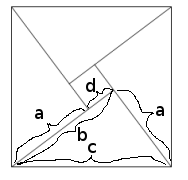
\includegraphics[width=0.4\linewidth]{images/p139_2.png}
    \end{figure}

    \begin{center}
        $d=b-a$ \\
        $c \equiv 0 \: \text{mod}\: d$
    \end{center}

\end{frame}

\begin{frame}
    \frametitle{Problema 139}

    \begin{table}[htpb]
        \centering
        \begin{tabular}{c c c}
            3        & 4        & 5 \\
            21       & 20       & 29 \\
            119      & 120      & 169 \\
            697      & 696      & 985  \\
            4059     & 4060     & 5741  \\
            23661    & 23660    & 33461  \\
            137903   & 137904   & 195025  \\
            803761   & 803760   & 1136689  \\
            4684659  & 4684660  & 6625109   \\
            27304197 & 27304196 & 38613965
        \end{tabular}
    \end{table}
\end{frame}


\begin{frame}
    \frametitle{Problema }

    \begin{center}
        \textit{
        }
    \end{center}
\end{frame}

\end{document}
